\section{Experiments}
\label{sec:expe}

In this part, we compare \Moca to the other existing tools for memory analysis. In a first time, we present their main differences in terms of portability
and capabilities. Then, we present two sequences of quantitative experiments, one that outlines the importance of the default parameters chosen for our tool
and the other that compares the precision and performance of all the tools.

\newpage

\subsection{Methodology}
\label{sec:exp-methodo}

%This section briefly discusses our experimental setup for the evaluation of
%\Moca.

Our main experiments were run on  machines from Grid5000 \Edel
cluster.
\DB{\Stremi or \Idfreeze / OMP\_NUM\_THREADS ?}
    As some state of the art tools can only run on AMD machines, we also run
    some of the experiment presented in section~\ref{sec:expe-ovh} on
    \Idfreeze machine from
    Digitalis.
    These machines hardware specification is summarized in
    \tbl{tab:hw}\footnote{Both platforms provides an online hardware description:\\
        \url{https://www.grid5000.fr/mediawiki/index.php/Grenoble:Hardware\#Edel}
     \\\url{http://digitalis.inria.fr/index.php/Idfreeze}}.

\begin{table}[htb]
    \centering
    \begin{tabular}{lp{1.1cm}rrp{1.35cm}p{1.1cm}}
        \toprule
        \multirow{3}{.8cm}{CPU}
        &  & \multicolumn{2}{c}{Vendor} & \multicolumn{2}{c}{Model} \\
        \cmidrule(lr){3-6}
        & \Edel  & \multicolumn{2}{c}{Intel} & \multicolumn{2}{c}{Xeon E5520} \\
        & \Idfreeze & \multicolumn{2}{c}{AMD} & \multicolumn{2}{c}{Opteron 6174} \\
        %& \Stremi & \multicolumn{2}{c}{AMD} & \multicolumn{2}{c}{Opteron 6164 HE} \\
        \midrule
        \multirow{3}{.8cm}{System totals}
        & & Nodes & Threads & Freq & Memory \\
        \cmidrule(lr){3-6}
        & \Edel   & $2$ & $8$ & \SI{2.27}{Ghz} & \SI{24}{Gib} \\
        & \Idfreeze & $8$ & $48$ & \SI{2.20}{Ghz} & \SI{256}{Gib}\\
        %& \Stremi & $2$ & $24$ & \SI{1.7}{Ghz} & \SI{48}{Gib}\\
        \midrule
        \multirow{3}{.8cm}{Per node}
        & & Cores & Threads & L3 Cache & Memory \\
        \cmidrule(lr){3-6}
        & \Edel   & $4$ & $4$ & \SI{8}{Mib} & \SI{12}{Gib} \\
        & \Idfreeze & $6$ & $6$  & \SI{12}{Mib} & \SI{32}{Gib} \\
        %& \Stremi & $6$ & $6$  & \SI{12}{Mib} & \SI{24}{Gib} \\
        \bottomrule
    \end{tabular}
    \caption{Hardware configuration of our evaluation system.}
    \label{tab:hw}
\end{table}

For every experiment, we deployed the same \emph{Debian} \emph{Jessie}
environment running a \texttt{Linux 3.16.0-4} with hyper threading was
disabled.

\begin{table}[htb]
    \centering
    \begin{tabular}{p{1.3cm}lcc}
        \toprule
        & & Mechanisms* & Architecture \\
        \cmidrule(lr){3-4}
        \multirow{4}{.8cm}{Portability}
        & \TABARNAC & Inst & Intel, AMD \\
        \addlinespace
        & \Mitos & PEBS + Inst & Intel \\
        \addlinespace
        & \MemProf & IBS & AMD \\
        \addlinespace
        & \Moca & PfI (+ Inst) & \textbf{Any}\\
        \midrule
        & & Granularity & superset \\
        \cmidrule(lr){3-4}
        \multirow{4}{.8cm}{Trace precision}
        & \TABARNAC & Page & \textbf{Page} \\
        & \Mitos & \textbf{Address} & None \\
        & \MemProf & \textbf{Address} & None \\
        & \Moca & \textbf{Address} & \textbf{Page} \\
        \midrule
        & & \multicolumn{2}{C{5cm}}{Time, Thread sharing, CPU**} \\
        \cmidrule(lr){3-4}
        \multirow{4}{.8cm}{Additional information}
        & \TABARNAC & \multicolumn{2}{C{5cm}}{Thread sharing} \\
        \addlinespace
        & \Mitos & \multicolumn{2}{C{5cm}}{Time + CPU} \\
        \addlinespace
        & \MemProf & \multicolumn{2}{C{5cm}}{\textbf{All}}  \\
        \addlinespace
        & \Moca & \multicolumn{2}{C{5cm}}{\textbf{All}} \\
        \bottomrule
    \end{tabular}
    \caption{Comparison of different memory traces tools.
        %\TABARNAC~\cite{Beniamine15TABARNACRR},
        %\Mitos~\cite{Gimenez14Dissecting},
        %\MemProf~\cite{Lachaize12MemProf} and \Moca.
        \\
        \emph{*~Inst: Binary instrumentation, PfI: Pagefault Interception}\\
        \emph{**~CPU on which the access occured}}
        \label{tab:tools-comp}
\end{table}

We evaluate \Moca by comparing it to the following state of the art tools. The first one,
\Mitos, is the tracing tool from MemAxes~\cite{Gimenez14Dissecting} and relies on Intel
PEBS technology. 
The second one, \TABARNAC~\cite{Beniamine15TABARNACRR}, is one of our previous contribution.
It is based on a Pin instrumentation, which traps all the memory accesses but 
only counts the number of time each thread accesses to each page.
Although this is less precise than the information collected by \Moca, it does not require
the management of large and complex data structures.
The third one, \MemProf~\cite{Lachaize12MemProf}, is designed to analyze NUMA
performance issues and relies on AMD IBS.
\tbl{tab:tools-comp} summarizes the main differences
between \Moca and these other memory profiling tools.

In the following sections, all the tools are
evaluated on each of the 10 \NPB~\cite{Jin1999}.
Each point in each plot is the average of at least $30$ executions. Along with each point,
the error bars represent the standard error.
Except for the experiment about the influence of \Moca's parameters, on each
experiment, \Moca has been run with it's default parameters: a wakeup interval of
\SI{0.5}{s} for the logging process and \SI{50}{ms} for the monitoring thread.


We consider experimental reproducibility as an important matter, therefore we
distribute\footnote{The three distribution are available on github:\\
    \url{https://github.com/dbeniamine/hpdc_expe}}
every file needed to reproduce our experiments at three different levels:
%First we distribute the filtered results (csv files) along with
%\texttt{R-markdown} scripts that generated the plots presented in this article
%to allow reproduction of our statistic analysis. The second level contains the
%full raw traces along with the script required to generate the filtered files
%of the first level and the analysis scripts. Finally we provide a git
%repository including our deployment  environment, dependencies to each tools
%and every files needed for the experiments and instruction on how to reproduce
%the experiments with and without access to grid5000.

\begin{enumerate}
    \item \textbf{Statistic analysis:} To reproduce our statistic analysis we provide
        the filtered results (csv files) from the experiment along with the
        \texttt{R-markdown} scripts that generated the plots presented in this
        article.
    \item \textbf{Raw analysis:} We also distribute the full raw traces
        generated by our experiments with the scripts used to extract the
        filtered traces and the analysis scripts.
    \item \textbf{Experiment reproducibility:} Finally we provide a git
        repository including our deployment environment, dependencies to each
        tools and every files needed for the experiments and instruction on
        how to reproduce the experiments with and without access to grid5000.
\end{enumerate}


%\subsection{Experiments}
\subsection{Moca default parameters}
\label{sec:expe-param}

Before comparing \Moca to existing tools, we need to evaluate the impact of
the wakeup intervals (logging daemon and monitor thread) on the trace
precision and on the overhead. To do so, we run the \IS benchmark instrumented by \Moca with
a wakeup interval ranging from \SI{0.1}{s} to  \SI{0.9}{s} for the logging daemon and from \SI{20}{ms} to
\SI{100}{ms} for the monitoring thread. For each run, we measure \IS execution time and the number of
accesses captured. We have chosen \IS for this evaluation as it is one of the memory intensive \NPB,
quick experiments with other ones confirmed these results. This experiment was
run on a machine from the \Edel cluster.

\begin{figure}[htb]
    \centering
    \begin{subfigure}{\linewidth}
        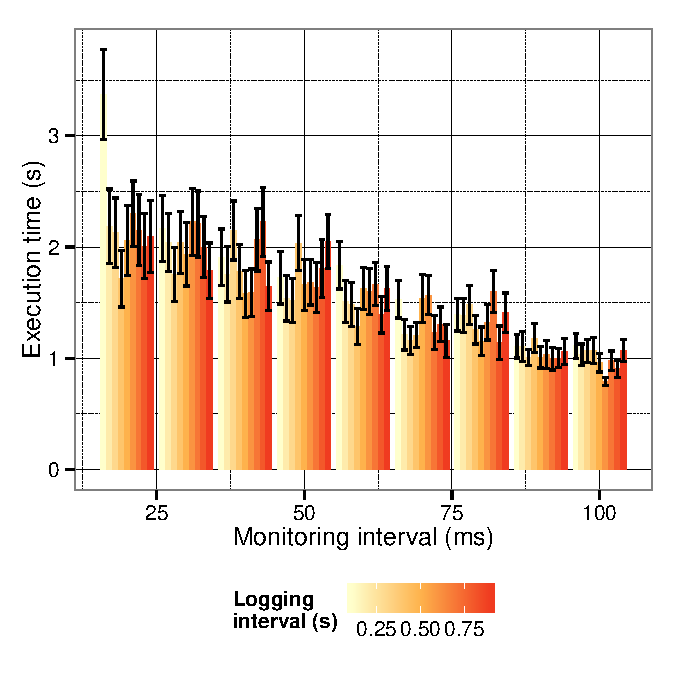
\includegraphics[width=\linewidth]{moca_param.pdf}
        \caption{Execution time.}
        \label{fig:param_time}
    \end{subfigure}
    \begin{subfigure}{\linewidth}
        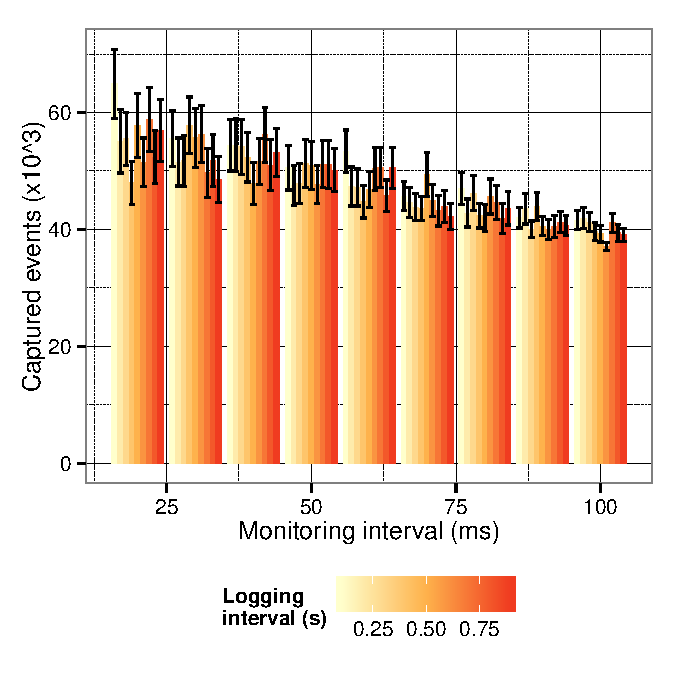
\includegraphics[width=\linewidth]{moca_param_events.pdf}
        \caption{Number of captured events.}
        \label{fig:param_evts}
    \end{subfigure}
    \caption{Influence of the wakeup intervals on \IS, class A.}
    \label{fig:param}
\end{figure}

We can see on the \fig{fig:param_time} that the execution time decreases when we
reduce the monitoring wakeup interval, at \SI{40}{ms}
it seems to reach its worst level, thus we should keep it larger. At \SI{50}{ms}, the
\fig{fig:param_evts} shows that we obtain more than two thirds of the events captured
at smaller intervals, which seems quite reasonable. Finally for this value, a logging
interval of \SI{0.5}{s} seems to provide a good trade-off  between
execution time and precision.
These two values have been chosen as default values in \Moca.


% \newpage

\subsection{Comparison with existing tools}
\label{sec:expe-ovh}

As preliminary experiments shows that \Mitos capture by
default way less events than \TABARNAC and \Moca, we also compare our tool to
\Mitos with a sampling period chosen to increase the number of pages
captured, We call this version \MitosTun.

Due to technical limitations \MemProf default sampling period have been
increased from  $0x8FFF0$ to $0x1FFFF0$ and the library used for retrieving
data structure information was disabled.
%\footnote{see \url{https://github.com/Memprof/scripts/issues/1}}

\DB{If new \MocaPin expe ok, update here}
% Finally our evaluation also differentiate \Moca (kernel module only) from
% \MocaPin which also retrieve the data structure information using a Pin
% instrumentation, we do this differentiation to evaluate the impact of Pin on
% \Moca performances.

We compare the different tools on two aspect: trace
precision and induced slowdown. The first experiment compares the tools on two
criteria:  the percentage of pages captured during the analysis. We use
\TABARNAC as a reference to compute this percentage as it is designed to
compute the number of accesses of each pages of the studied application. Then we
compare the tools in terms of number of captured events. We show the ratio
$\frac{captured\_events(tool)}{captured\_event(Moca)}$ as \Moca is usually the
tools that provides the more precise traces. We consider one event as one
timestamped access. According to this definition, \TABARNAC does not capture
any events as it only keep one counter per page and per thread without any
temporal informations. Thus \TABARNAC is excluded from this comparison.
The second experiment compare the
slowdown factor of the different tools.
%$slowdown\_factor(tool,bench)=\frac{exec\_time(bench,tool)}{exec\_time(bench)}$.
All these experiments have been run on each of the \NPB on class A.

\begin{figure}[htb]
    \centering
    \begin{subfigure}{\linewidth}
        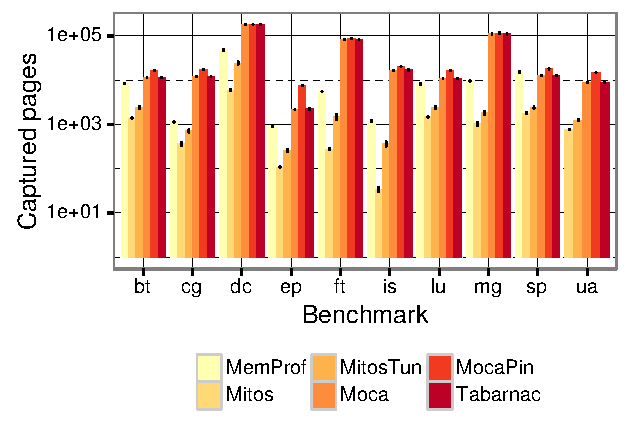
\includegraphics[width=\linewidth]{moca_pages_intel.pdf}
        \caption{Percentage of captured pages.}
        \label{fig:pages}
    \end{subfigure}
    \begin{subfigure}{\linewidth}
        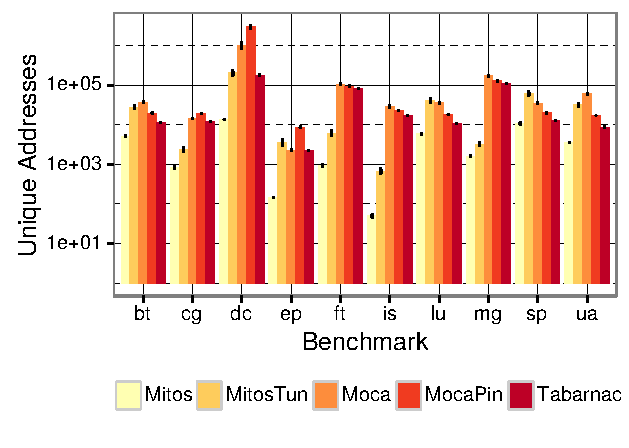
\includegraphics[width=\linewidth]{moca_addr_intel.pdf}
        \caption{Percentages of events captured (compared to \Moca).}
        \label{fig:addr}
    \end{subfigure}
    \caption{Precision of the traces generated by the different tools on the \NPB.}
    \label{fig:pages-addr}
\end{figure}

\fig{fig:pages-addr} presents the results of the precision evaluation of the
different tools. The values used for \Mitos, \MitosTun, \Moca and
\TABARNAC comes from runs on \Edel machines, while \MemProf results comes from
\Idfreeze.

We can see on \fig{fig:pages} that \Moca and \TABARNAC always capture exactly
\SI{100}{\%} of the accessed pages which is consistent with these tools
descriptions as both of them are designed to capture every pages of the
execution.

\Mitos usually collect less than $12.5\%$ of the pages, adding some fine tunning
can almost double this number but it still miss most of the address space.

Concerning \MemProf, it is important to note that we have increased the
default sampling period to overpass technical limitations. With this
modification we can see that \MemProf capture significantly more pages than
\Mitos and \MitosTun. For more than half of the studied applications it does
not see more than \SI{50}{\%} of the addresses space. For \BT, \LU and \UA
\MemProf manage capture around \SI{75}{\%} of the accessed pages. Finally for
\SP it seems to capture more pages than \TABARNAC and \Moca. As these two
tools uses two different methods to capture every page and provide the exact
same number of pages, we can guess that for \SP, which is not a memory
intensive benchmark, \MemProf capture some system noise in the trace.

From \fig{fig:addr} we can see that, as expected, for almost every benchmarks
\Moca collects significantly more events than the other tools.  The only
benchmark for which \Moca is not the more precise tool is \EP which is an
Embarrassingly Parallel application with very few memory accesses.  For almost
every other benchmarks both \Mitos (with or without tunning) and \MemProf
hardly reach \SI{10}{\%} of the accesses collected by \Moca, the only exception is
\CG for which \MemProf captures from \SI{25}{\%} to \SI{50}{\%} of the accesses
collected by \Moca.

These results proves that most existing tools can miss a considerable part of
the address-space while \Moca guarantee to provide a superset of the accessed
pages. Furthermore they show that \Moca is the only existing tool able to provide a
trace precise enough to have an overview an application's memory behavior. As
stated, not only our tool provide a complete trace at the granularity of the
page but it is also significantly more precise than the other existing tools in term of
number of unique addresses captured. Finally, adding a Pin instrumentation to
\Moca does not seems to disturb considerably the trace quality thus it seems
safe to use it.

\begin{figure}[htb]
    \centering
    \begin{subfigure}{\linewidth}
        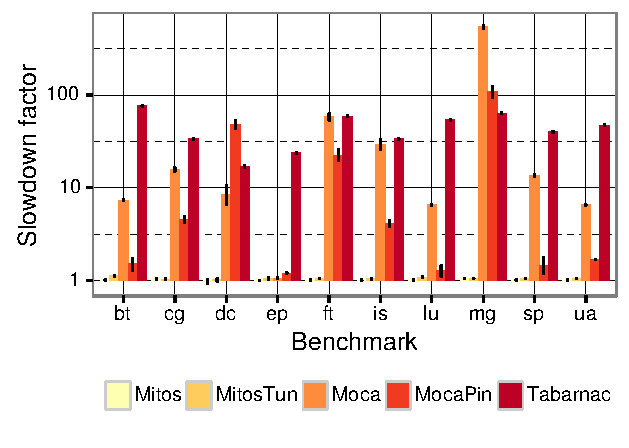
\includegraphics[width=\linewidth]{moca_overhead_intel.pdf}
        \caption{Evaluation on \Edel (Intel)}
        \label{fig:ovh-Intel}
    \end{subfigure}
    \begin{subfigure}{\linewidth}
        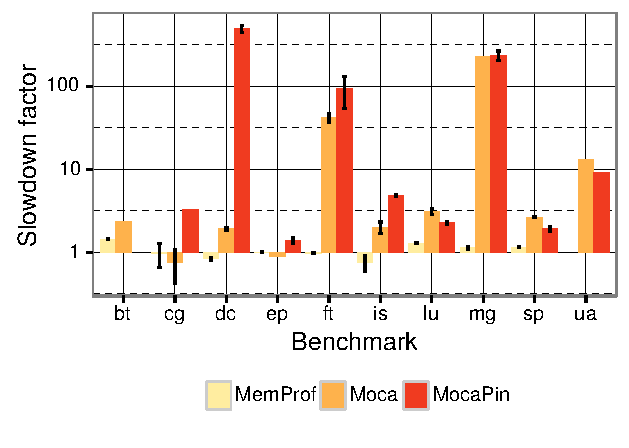
\includegraphics[width=\linewidth]{moca_overhead_amd.pdf}
        \caption{Evaluation on \Idfreeze (AMD)}
        \label{fig:ovh-AMD}
    \end{subfigure}
    \caption{Slowdown factor of \Moca on the \NPB compared to state of the art tools.
    Y-axis is in log scale.}
    \label{fig:ovh}
\end{figure}

\fig{fig:ovh} shows for each of the \NPB, the slowdown factor when
instrumented by \Moca and the other existing tools on Intel
(\fig{fig:ovh-Intel}) and AMD (\fig{fig:ovh-AMD}) Machines the Y-axis is in
log scale.

From \fig{fig:ovh-Intel}, we can see that \Mitos, \MitosTun overhead is
almost negligible which is not the case for \Moca and \TABARNAC, this
difference is explained by the results of the previous experiment, as these
tools usually collects less than \SI{10}{\%} of the accesses collected by \Moca and
miss a significant part of the address space.

We can classify the benchmarks into three groups:
for \BT, \CG, \EP, \LU, \SP and \UA, \Moca is
significantly faster than \TABARNAC. This set of benchmarks is interesting as it is made of varied application profiles.
Indeed, if \EP is mostly doing parallel computation with only a few number of
memory accesses, \CG is memory intensive and
\BT, \LU as well as \SP are pseudo applications doing a significant usage of memory.
And while \UA is categorised as \emph{unstructured computation,
parallel I/O and data movement} by the \NPB
website\footnote{\url{http://www.nas.nasa.gov/publications/npb.html}}, its
interactions with memory seems noticeable.

The second group only contains memory oriented benchmarks (\DC and \FT and
\IS). For this group, \Moca is as good as \TABARNAC or a bit faster, probably
because the balance between computations and memory accesses hides the
overhead of the instrumentation.

For the last benchmark: \MG, \Moca is significantly slower than \TABARNAC. This benchmark
seems to be a pathological case were the execution time with \Moca has a lot a
variability. By looking at our experiment logs, we found that \MG seems to
generate a lot of conflicts on \Moca false page fault hash map. A solution
could be to increase the size of this hash map which is quite difficult as
memory space in the kernel is limited, another easier solution would consist on
working on a smaller version of \MG and see if the analysis is still useful.

\DB{Update with new expe results}
\fig{fig:ovh-AMD} shows the results of the evaluation on the AMD machine
(\Idfreeze), it is important to note that this machine have $48$ threads which
is much more than the $8$ threads of \Edel cluster. This difference explain
the fact that for most benchmarks, \Moca overhead is way lower than on the
\Edel machines, and it shows that \Moca scale pretty well.
For its part \MemProf exhibit a slowdown factor comparable to \Mitos while
providing traces a little more precise than this tool but still incomplete and
way less precise as \Moca traces.

\subsection{Summary}
\label{sec:expe-cncl}

We have tested \Moca with various applications and using several parameters.
Our experiments, show that \Moca has a good behavior for a wide range of
parameter and helped us defining their default values. Our experiments also
show that, with these parameters, provides significantly more precise traces
than state of the art tools. Compared to the tools that provide comparable
(but still less precise traces) \Moca is at worst as slow as these tools and
often faster.  It is noteworthy that \Moca is the only tool able to provide a
detailed trace with temporal, spacial and sharing information while providing
guarantees on the information lost during the sampling.
